%%%%%%%%%%%%%%%%%%%%%%%%%%%%%%%%%%%%%%%%%%%%%%%%%%%%%%%%%%%%%%%%%%%%%%%%%%%%
% AGUJournalTemplate.tex: this template file is for articles formatted with LaTeX
%
% This file includes commands and instructions
% given in the order necessary to produce a final output that will
% satisfy AGU requirements, including customized APA reference formatting.
%
% You may copy this file and give it your
% article name, and enter your text.
%
%
% Step 1: Set the \documentclass
%
% There are two options for article format:
%
% PLEASE USE THE DRAFT OPTION TO SUBMIT YOUR PAPERS.
% The draft option produces double spaced output.
%

%% To submit your paper:
\documentclass[draft]{agujournal2019}
\usepackage{url} %this package should fix any errors with URLs in refs.
\usepackage{lineno}
\usepackage{color}
\graphicspath{ {figures/} }
\linenumbers
%%%%%%%
% As of 2018 we recommend use of the TrackChanges package to mark revisions.
% The trackchanges package adds five new LaTeX commands:
%
%  \note[editor]{The note}
%  \annote[editor]{Text to annotate}{The note}
%  \add[editor]{Text to add}
%  \remove[editor]{Text to remove}
%  \change[editor]{Text to remove}{Text to add}
%
% complete documentation is here: http://trackchanges.sourceforge.net/
%%%%%%%

\draftfalse

\journalname{JGR: Space Physics}


\begin{document}

\title{Statistical Properties of Electron Curtain Precipitation Estimated with AeroCube-6}

%% ------------------------------------------------------------------------ %%
%
%  AUTHORS AND AFFILIATIONS
%
%% ------------------------------------------------------------------------ %%

\authors{M. Shumko\affil{1,2}, A.T. Johnson\affil{1},  T.P. O'Brien\affil{3}, D.L. Turner\affil{4}, A.D. Greeley\affil{2}, J.G. Sample\affil{1}, J.B. Blake\affil{3}, L.W. Blum\affil{2}, A.J. Halford\affil{2}}


\affiliation{1}{Department of Physics, Montana State University, Bozeman, Montana, USA}
\affiliation{2}{NASA's Goddard Space Flight Center, Greenbelt, Maryland, USA}
\affiliation{3}{Space Science Applications Laboratory, The Aerospace Corportation, El Segundo, California USA}
\affiliation{4}{Johns Hopkins Applied Physics Laboratory, Laurel, Maryland, USA}


\correspondingauthor{M. Shumko}{msshumko@gmail.com}

\begin{keypoints}
\item The dual AeroCube-6 CubeSats are used to identify stationary, narrow in latitude, and persistent $>30$ keV precipitation termed curtains.
\item 90\% of the observed curtains in Low Earth Orbit are narrower than 20 kilometers in latitude.
\item Some curtains were continuously scattered into the atmosphere for multiple seconds.
\end{keypoints}


\begin{abstract}
Curtains are a recently discovered stationary, persistent, and latitudinally narrow electron precipitation phenomenon in low Earth orbit. Curtains are observed over consecutive passes of the dual AeroCube-6 CubeSats while their in-track lag varied from a fraction of a second to 65 seconds, with dosimeters that are sensitive to $> 30$ keV electrons. This study uses the AeroCube-6 mission to quantify the statistical properties of 1,634 curtains observed over three years. We found that many curtains are narrower than 10 kilometers in latitude with 90\% narrower than 20 kilometers, corresponding to a few hundred kilometer radial size at the magnetic equator. We examined the magnetic local time and geomagnetic dependence of curtains. We found that curtains are observed in the late morning and midnight magnetic local times, with a higher occurrence rate at midnight, and curtains are observed more often during \textcolor{blue}{geomagnetically active times (times of enhanced Auroral Electrojet)}. \textcolor{red}{Remove? $\rightarrow$} We tested the hypothesis that curtains are drifting remnants of microbursts. We found a few curtains in the bounce loss cone region in the north Atlantic Ocean, whose electrons were continuously scattered for at least 6 seconds as shown in one example. Such observations suggest that continuous curtain precipitation may be a significant source of $> 30$ keV electrons into the atmosphere, possibly scattered by a parallel direct current electric field.
\end{abstract}

\section{Plain Language Summary}
Electron curtain precipitation from space into Earth's atmosphere is a recently-discovered phenomenon observed by dual-spacecraft missions such as the AeroCube-6 CubeSats that orbit 700 kilometers above Earth's surface. Curtains appear stationary, remaining unchanged from seconds to a minute. Curtains are also very narrow along the satellite orbit (mostly in latitude). Besides these two properties, curtains and their impact on the magnetosphere and atmosphere are not well understood. Therefore, we used the AeroCube-6 mission that took data together for three years, to statistically quantify curtain properties and to better understand their origin. We found 1,634 curtains and found that 90\% of curtains are narrower than 20 kilometers in latitude, curtains are observed on the outer radiation belt field lines, and curtains are observed when the magnetosphere is disturbed. Curtains observed in a special region in the North Atlantic Ocean shed light on their origin. A few dozen curtains observed in this North Atlantic region were continuously precipitating into the atmosphere for multiple seconds, and are unlikely to be drifting. Therefore, curtains may be a significant source of atmospheric ionization responsible for the natural depletion of ozone.

\section{Introduction} \label{intro}
Curtain electron precipitation is a stationary phenomenon observed in low Earth orbit (LEO). Curtains are narrow in latitude and appear persistent for up to a minute between subsequent satellite passes. Curtains were recently discovered by \citeA{Blake2016} using the $> 30$ keV electron dosimeters onboard the dual AeroCube-6 (AC6) CubeSats that operated together between 2014 and 2017. This discovery was possible due to AC6's actively maintained in-track separation that varied between a few hundred meters and a few hundred kilometers. Besides the \citeA{Blake2016} study, not much is known about curtains including what they are, how are they generated, and their impact on the atmosphere. Answering these questions is an essential next step towards a more complete understanding of how curtains, and particle precipitation in general, affect the magnetosphere and Earth's atmosphere.

In low Earth orbit, curtains are narrower than a few tens of kilometers in latitude. A polar-orbiting LEO satellite, such as AC6, will pass through their cross-section in a few seconds; curtains appear in the electron count time series as short enhancements in flux. AC6 also observes similar-looking transient precipitation called electron microbursts. \textcolor{blue}{(Check with Lauren)} The microburst and curtain fluxes are enhanced in the AC6 data for different reasons: microbursts are short-lived, while curtains are narrow in latitude. Hence AC6, and other recently developed multi-spacecraft missions, are necessary to identify and distinguish between the transient microbursts precipitation and the persistent curtain precipitation.

Since the mid-1960s, microbursts have been observed by high altitude balloons where they appear as sharp peaks in flux with a sub-second duration \cite<e.g.>{Anderson1964, Brown1965_2, Parks1967}. Because balloons are relatively stationary, a microburst is easily classified as a transient phenomenon. Microburst electrons have also been directly observed by LEO satellites such as The Solar Anomalous and Magnetospheric Particle Explorer \cite<e.g.>{Blake1996, Lorentzen2001a, O'Brien2003, Douma2017}. But precipitation that looks like a microburst from a single LEO satellite is ambiguous---it can be transient, stationary and narrow in latitude, or both. Thus, multi-spacecraft missions such as the Focused Investigations of Relativistic Electron Burst Intensity, Range, and Dynamics (FIREBIRD-II) \cite{Crew2016, Johnson2020} and AC6 \cite{Blake2016, O'brien2016} are necessary to resolve the temporal vs. spatial ambiguity. \textcolor{red}{Remove the following sentence?} While this study focuses on curtain precipitation, microburst precipitation observed by AC6 was studied in \citeA{Shumko2020}.

\textcolor{red}{Rework this P?} The impact of microbursts on the outer Van Allen radiation belt and Earth's atmosphere may be substantial. \citeA{Lorentzen2001b}, \citeA{Thorne2005}, \citeA{Breneman2017}, and \citeA{Douma2019}---among others---estimated that microbursts could deplete the outer radiation belt electrons in about a day. Furthermore, \citeA{Seppala2018} modeled a 6-hour microburst storm and concluded that microbursts depleted mesospheric ozone by roughly 10\%. However, the impact of curtains is unknown, so it is crucial to understand the connection, if any, between microbursts and curtains. \textcolor{red}{Delete? $\rightarrow$} Curtains and microbursts can be easily misidentified from a single spacecraft so we may need to reevaluate single-satellite microburst studies. If curtains are numerous, then the atmospheric and magnetospheric impact associated with microburst observations from single sattelites may be overestimated.

\citeA{Blake2016} proposed a hypothesis that curtains are drifting remnants of microbursts. If a microburst is not completely lost in the atmosphere after the initial scatter, the remaining microburst electrons will spread out (bounce phase disperse) along the entire magnetic field line over a few bounce periods. Concurrently these electrons drift to the east, with higher energy electrons drifting at a faster rate. Assuming this hypothesis, the initially localized microburst is also spread out in longitude into the shape of a curtain. A similar phenomena was hypothesized by \citeA{Lehtinen2000} who predicted that drifting curtains can be created by energetic runaway beams driven by lightning, but these curtains will be observed at relatively low L shells.

\textcolor{red}{Check this} Precipitation bands, sometimes also referred to as spikes \cite<e.g.>{Imhof1991}, is another form of precipitation that can be related to curtains. Precipitation bands are stationary and were observed to persist from an hour to as much as half a day \cite<e.g.>{Brown1972, Blake1996}. \citeA{Blum2013} identified two precipitation bands and estimated that only 20 precipitation bands can deplete the outer radiation belt electrons. The mechanism responsible for scattering precipitation band electrons at high L is believed to be field line curvature scattering, \textcolor{red}{but the scattering mechanism for band electrons at lower L shells is currently unknown (is this true?)}, but has been hypothesized to be related to wave-particle interactions or acceleration due to a parallel direct current potential \cite{Hoffman1968}. 

This study expands on \citeA{Blake2016} by examining the statistical properties of curtains. We use 1634 confirmed curtain observations to study the distributions of the curtain: width in latitude, the geomagnetic conditions favorable to curtains, and the curtain distribution in L and magnetic local time (MLT). Lastly we will show examples of curtains that continuously precipitated in the bounce loss cone (BLC) region.

\section{Instrumentation} \label{instrumentation}
The AC6 mission was a pair of 0.5U (10x10x5 cm) CubeSats built by The Aerospace Corporation and designed to measure the electron and proton environment in low Earth orbit \cite{O'brien2016}. AC6 was launched on 19 June 2014 into a 620x700 km, $98^\circ$ inclination orbit. The AC6 orbit over the three year mission lifetime was roughly dawn-dusk, and precessed only a few hours in MLT: 8-12 MLT in the dawn and 20-24 MLT in the dusk sectors. The two AC6 spacecraft, designated as AC6-A and AC6-B, separated after launch and were in proximity for the duration of the three-year mission---maintained by an active attitude control system. The attitude control system allowed them to precisely control the amount of atmospheric drag experienced by each AC6 unit using the surface area of their solar panel ``wings." By changing their orientation, AC6 was able to maintain a separation between 2-800 km, confirmed by the Global Positioning System. The two AC6 units were in a string of pearls configuration, so one unit, typically unit A, was leading the other by an in-track lag: the time it would take the following spacecraft to catch up to the position of the leading spacecraft. To convert between the AC6 in-track separation and in-track lag, the AC6 orbital velocity was used. AC6's orbital velocity was $7.6$ km/s and varied by as much as $0.1$ km/s. The in-track lag was readily available with the Global Positioning System, which makes it easy to study precipitation phenomena observed at the same time, and at the same position by shifting one time series by the in-track lag.

Each AC6 unit contains three Aerospace microdosimeters (licensed to Teledyne Microelectronics, Inc) that measure the electron and proton dose in orbit \cite{O'brien2016}. The dosimeter used for this study is dos1 with a $> 30$ keV integral electron response, as the other dosimeters either responded primarily to protons or were not identical between unit A and B. All dosimeters sample at 1 Hz in survey mode, and 10 Hz in burst mode. 10 Hz data was readily available from both AC6 units from June 2014 to May 2017 while their in-track lag was less than 65 seconds. Figure \ref{a_10Hz_dist} shows the distribution of 10 Hz data as a function of AC6 in-track lag. The variety of AC6 separations and data availability over the three-year mission makes it possible to study transient electron microburst precipitation \cite{Shumko2020} and now stationary electron curtain precipitation.

\section{Methodology} 
\subsection{Curtain Identification} \label{curtain_identification}
The 10 Hz data was used to identify curtains with two criteria that are described below: a high spatial correlation, and prominently peaked. Before we applied the identification criteria, the AC6-B time series was shifted by the in-track lag to spatially align it with the AC6-A time series. 

The first identification criterion is a 1-second rolling Pearson correlation applied to both time series. Spatial features with a correlation greater than 0.8 are considered highly correlated. The second criterion is applied to any features that are highly correlated, to check if they are also prominently peaked. To find peaked precipitation, we used a method similar to the method used by \citeA{Blum2015} to identify precipitation bands and by \citeA{Greeley2019} to identify microbursts. Our method quantified the number of Poisson standard deviations, $\sigma$, that a dos1 count rate is above a 10-second centered running average, $B_{10}$. Locations where dos1 is at least two $\sigma$ above $B_{10}$, in other words $dos1 > 2\sqrt{B_{10}} + B_{10}$, are considered prominently peaked. 

We tuned the detection parameters to identify many candidate curtains while being feasible to check every detection. One author visually inspected 6,149 candidate curtains and 1,634 quality curtains were confirmed. Four curtain examples are shown in Fig. \ref{fig1}. In each example, the unmodified time series is shown in the top row and the spatially-aligned time series the bottom row. The in-track lag used to shift the bottom row is annotated by $dt$, corresponding to an AC6 in-track separation annotated by $s$. The bottom row shows highly correlated curtains observed at the same location for at least 3 to 26 seconds.

\begin{figure}
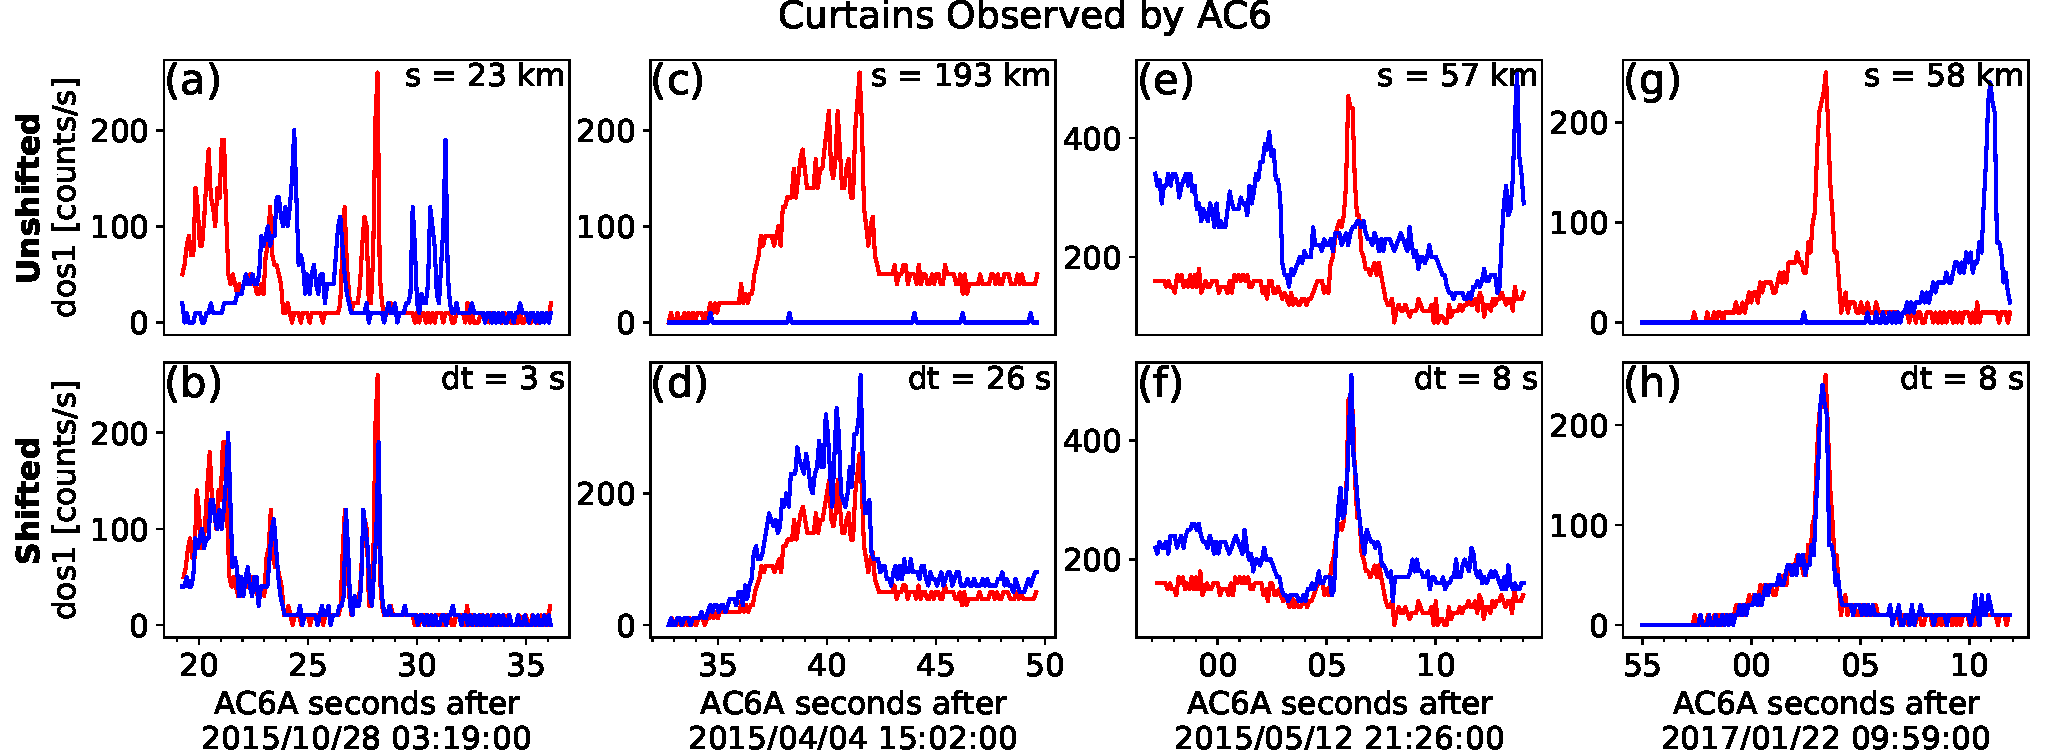
\includegraphics[width=\textwidth]{fig1.pdf}
\caption{Four examples showing the $>30$ keV electron time series data taken by AC6 at the same time (unshifted) in the top row and at the same position (shifted by dt seconds) in the bottom row. AC6-A, whose data is shown with red curves, was $s$ kilometers ahead of AC6-B. To show the data at the same position the AC6-B time series was shifted by the in-track lag annotated by dt. These examples show that curtain precipitation was highly correlated for up to 26 seconds.}
\label{fig1}
\end{figure}

\subsection{Differentiating Between Drifting and Precipitating Curtains}

The AC6 dosimeters lack the necessary pitch angle resolution to differentiate between drifting and precipitating electrons to test the \citeA{Blake2016} hypothesis that curtains are the drifting remnants of microbursts. Fortunately, one common method of distinguishing between precipitating, drifting, and trapped particles is using particle measurements in conjunction with the location of the South Atlantic Anomaly (SAA).

Earth's magnetic field is asymmetric, which creates a region of weaker magnetic field in the South Atlantic Ocean called the South Atlantic Anomaly. The weaker magnetic field in the SAA naturally differentiates particles by pitch angle into trapped and quasi-trapped populations. While some particles observed in LEO are trapped and will execute closed drift paths, most particles observed in LEO are quasi-trapped: they drift around the Earth until they reach the SAA. Within the SAA, the weaker magnetic field strength can lower the particle's mirror point altitude into the atmosphere, where collisions with the atmospheric ions are more numerous and the particle is lost. 

Particles that are quasi-trapped have pitch angles in the drift loss cone and will precipitate within one drift period (often within the SAA). Particles with smaller equatorial pitch angles (less than $\approx 6^\circ$) that are lost in the atmosphere within one bounce are in the bounce loss cone (BLC). Traditionally, we define a BLC particle if its mirror point altitude is at or below 100 km in either hemisphere.

In most regions outside of the SAA and its conjugate point in the North Atlantic, AC6 will observe a combination of drift and bounce loss cone electrons. In the SAA, AC6 does not only observe electrons that are immediately lost, but a combination of electrons that are in the drift loss cone, bounce loss cone, and trapped (a trapped electron that locally mirrors at AC6's altitude in SAA will mirror at higher altitudes everywhere else). In the region magnetically conjugate to the SAA in the North Atlantic, AC6 only observes electrons in the BLC. Here, if an electron makes it to AC6's altitude, it might be in the local loss cone and precipitate in the local hemisphere. Alternatively, the electron can mirror at or below AC6 and bounce to its conjugate mirror point deep in the atmosphere or below sea level in the SAA. Therefore, any electrons observed in the BLC region must rapidly precipitate. 

We estimated the BLC region for locally-mirroring electrons in the North Atlantic Ocean using the IRBEM-Lib magnetic field library and the Olson-Pfitzer magnetic field model \cite{irbem, Olson1982}. We defined a latitude-longitude grid, with a $\approx 0.5^\circ \times 0.5^\circ$ grid size, spanning the North Atlantic at 700 kilometer altitude (a typical altitude for AC6), and estimated the local magnetic field strength. For each latitude-longitude point we traced the magnetic field line to the southern hemisphere and found the conjugate mirror point altitude. If the conjugate mirror point is at or below 100 kilometers, the electron is likely lost and the assosiated grid point is considered to be in the BLC. Furthermore, a more rigorous bounce loss cone criterion is the conjugate mirror point altitude below sea level. In this case, the electron is definitely lost. Since AC6 can measure locally-mirroring electrons in the North Atlantic, the spacecraft altitude determines the upper bound conjugate mirror point altitude in the SAA. The BLC region estimated by this method closely matches the BLC region shown in \citeA[Figure 1]{Comess2013} and \citeA[Figure 3]{Dietrich2010}. Furthermore, we repeated the same analysis using the Tsyganenko 1989 model \cite{Tsyganenko1989}, which yielded similar boundaries.

\section{Results} \label{results}
\textcolor{red}{Remove the enumerated list?}
In this study we answered three questions:

\begin{enumerate}
\item What is the distribution of curtain widths in latitude?
\item When and where are curtains observed?
\item Are curtains drifting or locally precipitating?
\end{enumerate}

\subsection{Curtain Width}
We quantified the curtain width in the dos1 time series as the width at half of the curtain's topographic prominence: the height of the peak above the lowest contour that encircles the peak but contains no higher peak. Examples of curtains and their widths are shown in Appendix B. The spatial width of a curtain is then the product of the observed width in time and AC6's orbital velocity. The curtain width is measured along AC6's orbit track which is mostly in latitude, therefore the estimated curtain widths are also mostly in latitude. The distribution of curtain widths is shown in Fig. \ref{width_dist}. Curtains are very narrow. Many curtains are narrower than 10 km in latitude, and 90\% are narrower than 20 km in latitude.

\begin{figure}
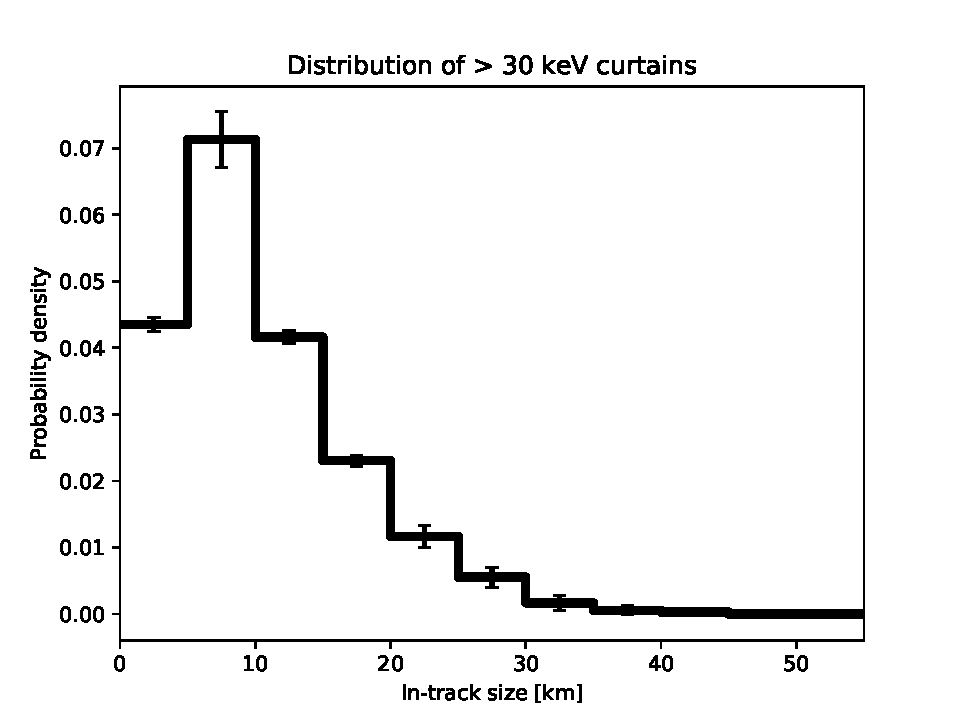
\includegraphics[width=\textwidth]{ac6_curtain_width_dist.pdf}
\caption{The distribution of curtain width in latitude. The error bars are derived assuming the Poisson standard error.}
\label{width_dist}
\end{figure}

\subsection{When and Where Are Curtains Observed}
The distribution of curtains in L and MLT is shown in Fig. \ref{l_mlt_dist}. Figure \ref{l_mlt_dist}a shows the distribution of the observed curtains while Fig. \ref{l_mlt_dist}b shows the same distribution normalized by the number of quality 10 Hz samples that AC6 took at the same location in each L-MLT bin. This normalization is shown in Fig. \ref{l_mlt_dist}c. The normalized curtain distribution in Fig. \ref{l_mlt_dist}b shows an enhanced curtain occurrence in the outer radiation belt in late morning and midnight MLT regions.

We also quantified the geomagnetic conditions favorable for curtains. Figure \ref{ae_dist}a shows the distribution of the minute cadence Auroral Electroject (AE) index between 2014 and 2017 in solid black. Furthermore, the distribution of the AE index when curtains were observed is shown by the solid blue lines. Curtains are observed during both low and high geomagnetic activity, slightly more often at higher AE than the idex itself (curtain distribution trends above the AE index when $AE > 200$). Lastly, we normalized the curtain distribution in Fig. \ref{ae_dist}a assuming an unrealistic, but insightful, scenario where any AE index is equally probable. The normalized curtain distribution is shown in Fig. \ref{ae_dist}b, which emphasizes that the curtain occurrence frequency increases with AE index.

\begin{figure}
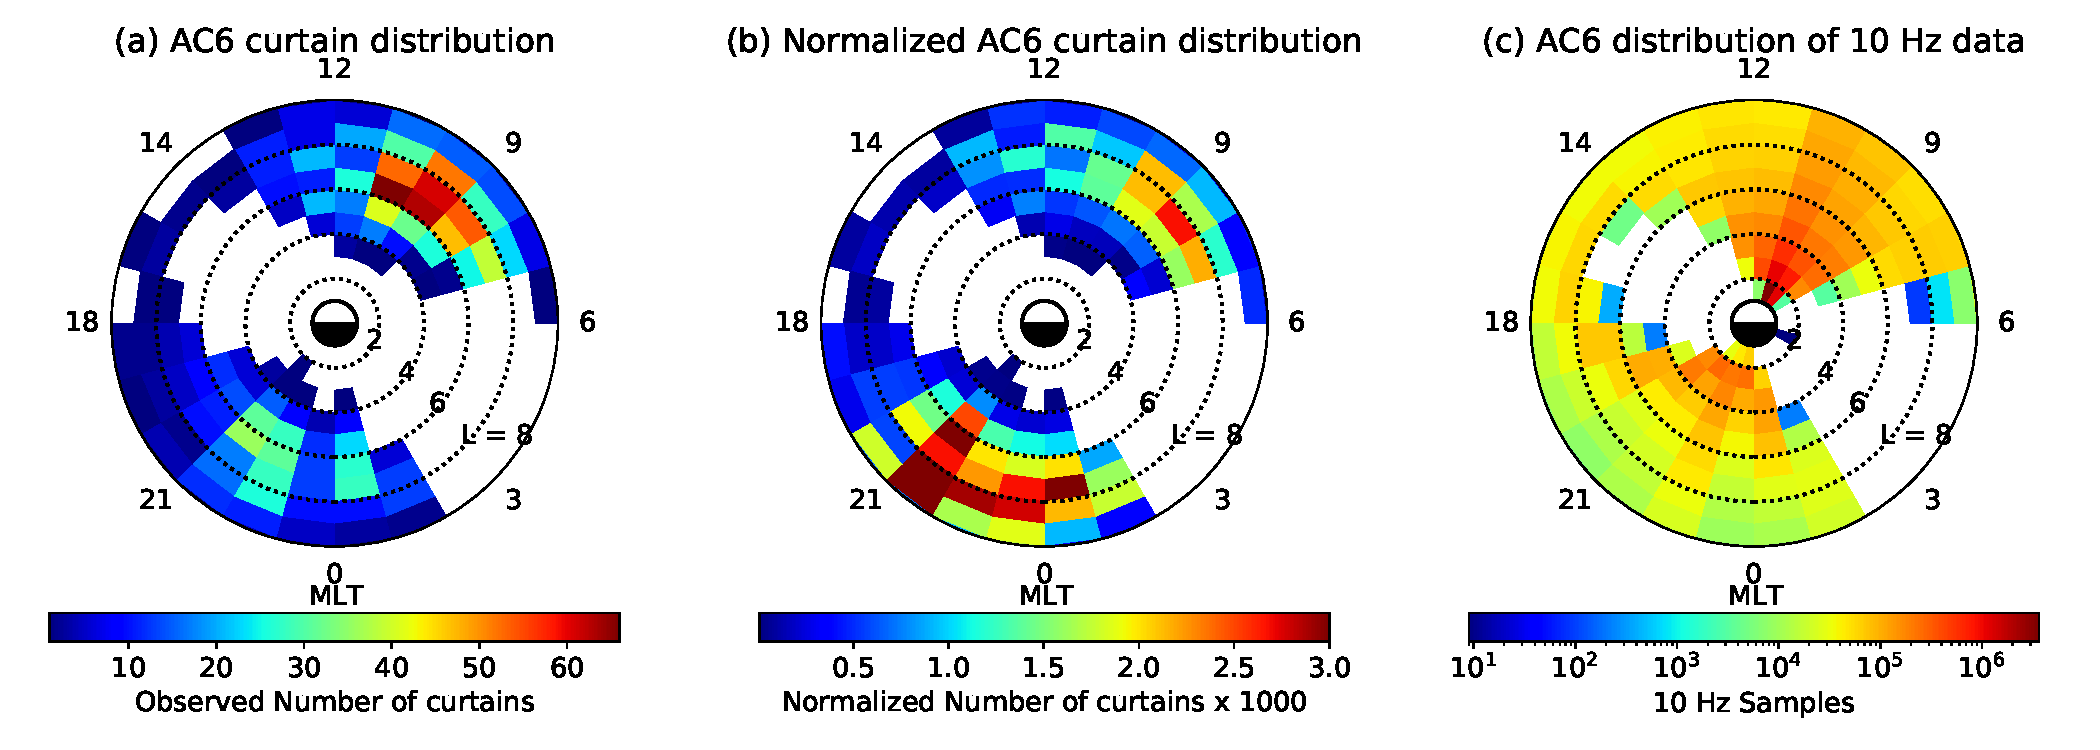
\includegraphics[width=\textwidth]{fig2_3.pdf}
\caption{The distribution of observed curtains by L shell and MLT. Panel a shows the locations of all observed curtains used in this study. Panel b shows the curtain distribution normalized by the number of quality 10 Hz samples taken in each bin, shown in panel c. The white bins in panels a and b show where no curtains were observed. In panel c the white bins show where AC6 did not take any 10 Hz data at the same location.}
\label{l_mlt_dist}
\end{figure}

\begin{figure}
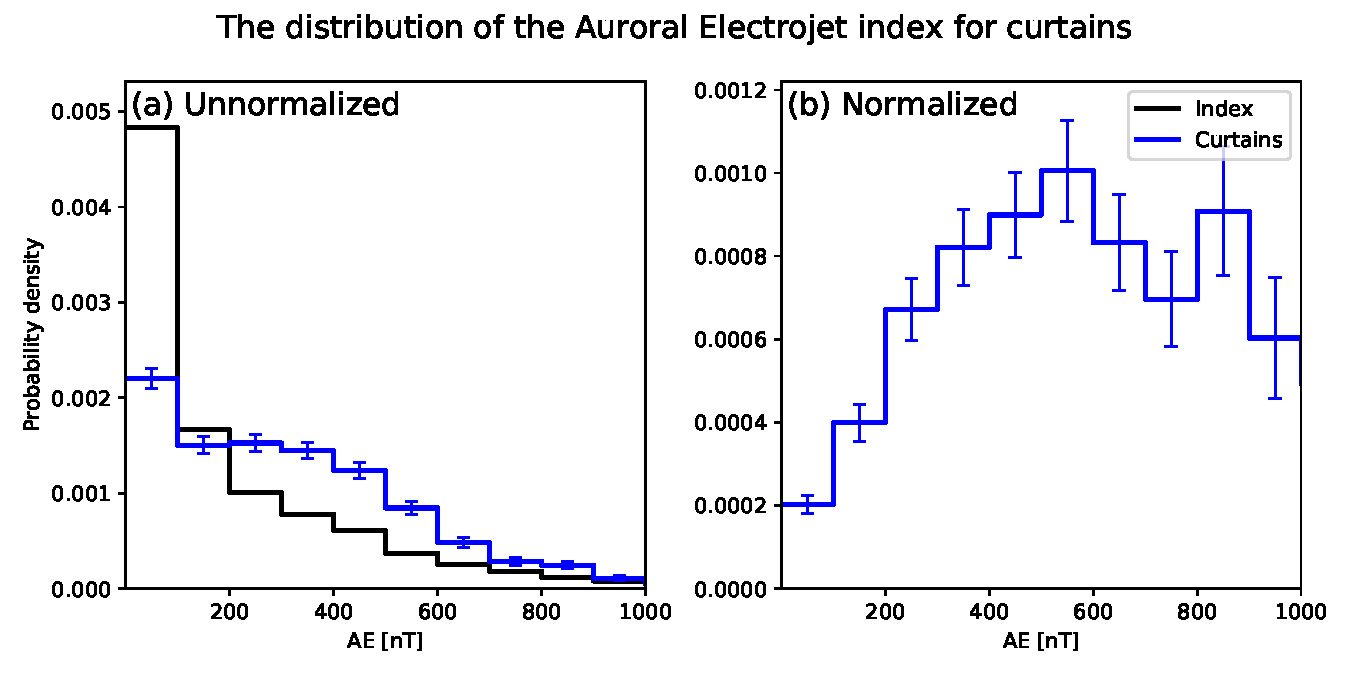
\includegraphics[width=\textwidth]{ac6_curtain_AE_dist.pdf}
\caption{The distribution of the Auroral Electroject (AE) index when curtains were observed. The blue line in panel a shows the distribution of AE when curtains where observed, and for reference the black line is shows the distribution of the AE index itself between 2014 and 2017. Panel b shows the curtain distribution normalized by the AE index, and it represents the distribution assuming that any AE index is equally probable. The error bars are derived assuming the Poisson standard error.}
\label{ae_dist}
\end{figure}

\subsection{Local Atmospheric Precipitation}
Lastly we investigate if curtains are drifting or locally precipitating. Figure \ref{fig3}a shows a map of the northern BLC region in the North Atlantic. The solid blue line is the northern boundary where an electron that mirrors locally at 700 km has a conjugate mirror point at 100 km in the SAA. Immediately south of the solid blue line, the conjugate mirror altitude rapidly decreases towards, and below, sea level. The dashed blue line is the boundary where the conjugate mirror point altitude is at sea level. South of this line the mirror point is inside the Earth. For reference, AC6 takes about 30 seconds to move between the solid and dashed blue curves. The two dotted black curves in Fig. \ref{fig3}a are roughly the boundary of the outer radiation belt, defined as $\mathrm{L}=4-8$.

We found 36 curtains that were observed inside the BLC region. Figure \ref{fig3}b-e shows 4 curtain examples (AC6-B time shifted by the in-track lag), along with the AC6 in-track lag, L and MLT during the observations annotated. The AC6 locations where these curtains were observed are shown in Fig. \ref{fig3}a with the red stars and the corresponding panel labels.

\begin{figure}
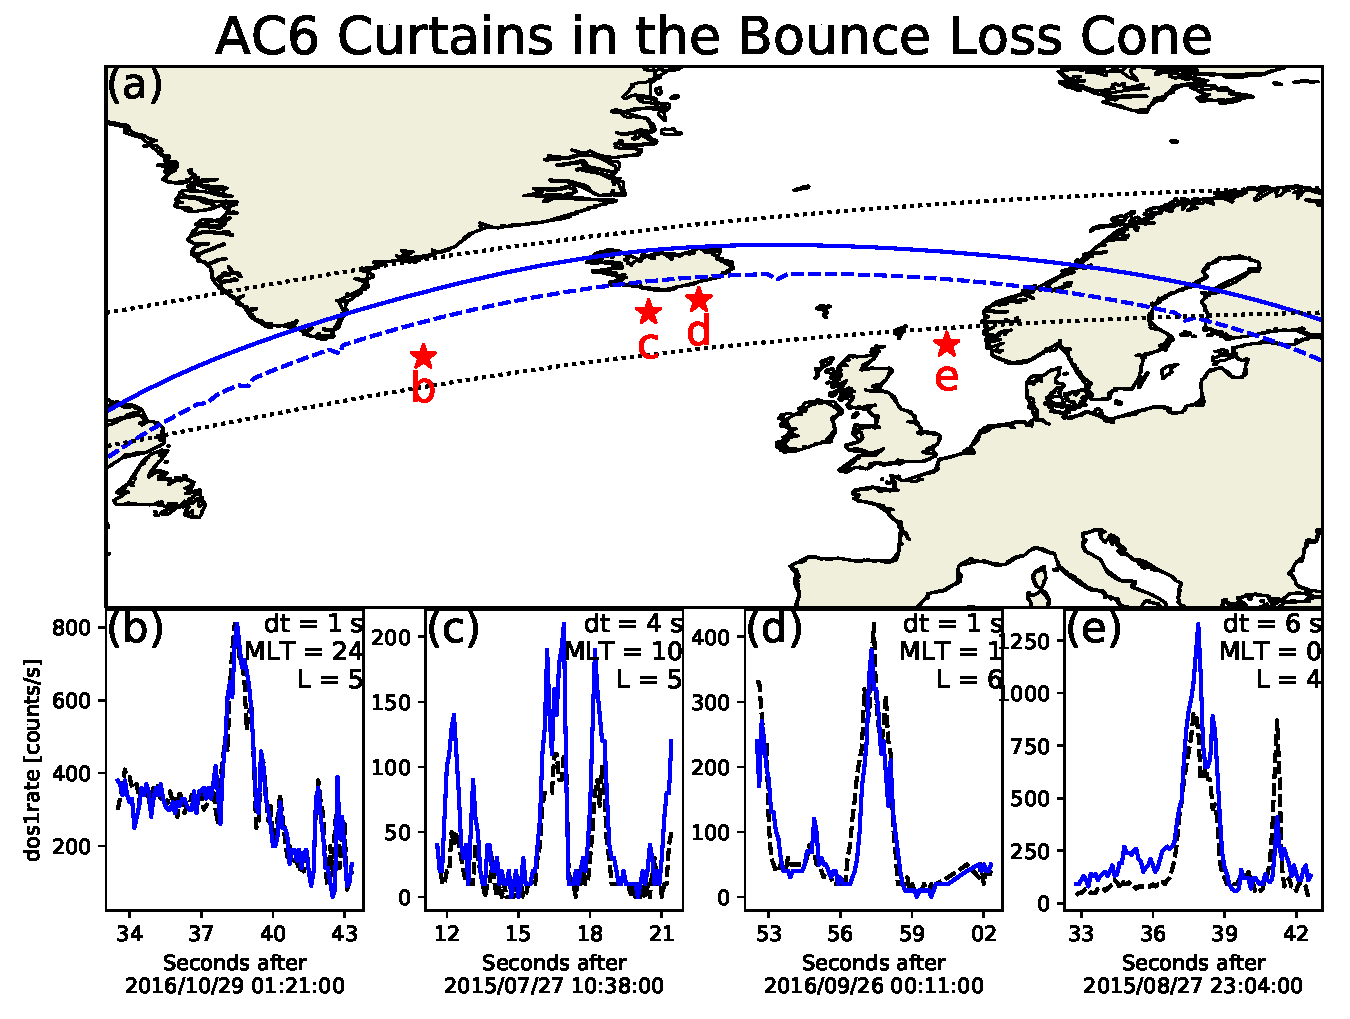
\includegraphics[width=\textwidth]{fig3.pdf}
\caption{Curtains observed in the bounce loss cone region. Panel a shows a map of the North Atlantic region with the outer radiation belt, defined by $L=4-8$, shown with the dotted black curves. The solid blue curve shows the northern boundary of the bounce loss cone region. Along this curve, electrons locally mirroring at 700 kilometers altitude have a conjugate mirror point at 100 kilometers altitude in the SAA. A more strict bounce loss cone criterion is the dashed blue curve that represents a conjugate mirror point altitude at sea level in the SAA. The 4 red stars with labels show the locations of the curtain examples shown in the corresponding panels b-e. The panels b-e show the 4 example curtains with the AC6-A data shown by the red line and the time-shifted AC6-B data with the blue line. AC6-A was ahead in all examples except panel d.}
\label{fig3}
\end{figure}

\section{Discussion} \label{discussion}
\subsection{Curtain Width}
Curtains are very narrow in latitude. Figure \ref{width_dist} shows that the width of most curtains is on the order of 10 kilometers and 90\% are narrower than 20 km. Scaled to the magnetic equator, where we presume curtains are generated, these widths correspond to a source with a radial scale size of a few hundred kilometers. As shown in Fig. \ref{fig1}, it is remarkable that some curtains remain stationary and maintain a fine structure after multiple seconds with little observable difference. However, some curtains appear to be slightly and systematically shifted in latitude, while maintaining their fine structure (not shown).

If curtains are remnants of microbursts, then the distribution of curtain widths in latitude, shown in Fig. \ref{width_dist}, should correspond to the microburst size distribution. The curtain width distribution is qualitatively similar to the size distribution of microbursts estimated in \citeA{Shumko2020}. However, a thorough quantitative comparison is not done here because there are at least two sources of bias that need to be addressed: as argued in \citeA{Shumko2020}, microbursts observed simultaneously by AC6 must be larger than the spacecraft separation; and the detection algorithm described in section \ref{curtain_identification} loses sensitivity for wider curtains. For curtains with a width similar to the detection algorithm's 10-second baseline, the baseline will be elevated making the curtain peak less pronounced. Both biases underestimate the microburst size and curtain width distributions, but we believe that they are likely too small to significantly change these results.

\subsection{When and Where Are Curtains Observed}
Figure \ref{l_mlt_dist}b shows that curtains likely originate in the outer radiation belt and are observed relatively more in the late evening than late morning regions. Furthermore, are likely observed at higher L shells near midnight MLT, however the sampling statistics at high L are rather limited because AC6 rapidly crosses high L shells. Nevertheless, Fig. \ref{l_mlt_dist}b hints that curtains near midnight MLT were observed to L shells possibly outside the outer radiation belt. Lastly, Figure \ref{ae_dist} shows that curtains are associated with an enhanced AE.
 
\subsection{Curtains Observed in The Bounce Loss Cone}
The curtains that were observed in the bounce loss cone and shown in Fig. \ref{fig3} cast doubt on the microburst-curtain hypothesis described in the introduction. These curtains were observed near the sea level mirror altitude curve, thus they were not drifting and were precipitating for as long as 6 seconds, as shown in Fig. \ref{fig3}e. The curtain precipitation persisted for multiple bounce periods ($\approx 1.5$ seconds for 30 keV electrons in this region). This is a surprising result because there are relatively few mechanisms capable of persistently scattering electrons. This mechanism must be radially localized near the magnetic equator, on a scale of a few hundred kilometers. A candidate mechanism is a direct current electric field that is parallel to the background magnetic field that lowers the electron mirror point to AC6 altitudes. To find the minimum potential we assume the electron is barely trapped and has a 100 kilometer conjugate mirror point altitude in the SAA, so initially the electron will mirror above AC6 in the bounce loss cone region. 

To find the parallel potential, $q \Phi$,  we use the kinetic energy, $W$, of a $30$ keV electron at its initial mirror point with a magnetic field strength of $B_i$. The kinetic energy at the initial mirror point can be written as $W_i = \mu B_i$ where $\mu$ is the first adiabatic invariant that is conserved during this acceleration. When a parallel potential acts on the electron of charge $q$ and does $q \Phi$ amount of work the electron will mirror closer to Earth's surface and mirror at a field strength $B_f$ where its final energy is $W_f = \mu B_f$. Now we relate the initial and final kinetic energy of the electron,

\begin{equation}
\mu B_f = \mu B_i + q \Phi.
\end{equation} Then we solve for $q \Phi$ and substitute $\mu$ to express the above equation as a function of the initial kinetic energy 

\begin{equation}
 q \Phi = W_i \frac{(B_f - B_i)}{B_i}.
\end{equation} The parallel potential is proportional to $W_i$ so a larger potential is necessary to accelerate higher energy electrons. AC6 dos1 electron energy response increases rapidly from 30 keV to a peak at 100 keV \cite<Figure 2 in>{O'brien2019}, therefore our assumption that $W_i = 30$ keV will underestimate the parallel potential. In reality, the counts observed by AC6 is a convolution of, among other things, the AC6 dos1 electron energy response and the falling electron energy spectrum. Thus, the majority of electrons that AC6 observed have energies close to 30 keV and the $W_i = 30$ is an appropriate approximation.

We again used IRBEM-Lib to estimate $ q \Phi$. For each example curtain in Fig. \ref{fig3}, we first estimated the local magnetic field, $B_f$, that the electron descended to after the acceleration. Then we traced the local field line into the SAA. We estimated $B_i$ at 100 kilometers altitude in the SAA for barely trapped electrons. With the initial and final $B$, along with $W = 30$ keV, the minimum potential was between $q \Phi = 1-4$ kV for the 4 examples shown in Fig. \ref{fig3}. 

The range of estimated potentials is typical for the aurora. \citeA{Partamies2008} used the observations made by the Fast Auroral SnapshoT (FAST) mission and reported that the auroral inverted-V electron precipitation structures, with electron energies up to a few tens of keV, were accelerated by 2-4 kV parallel potentials. The inverted-V structure and curtains share a number of similarities including: their energy, latitudinal width, and high occurance rate in the midnight MLT region. A possible connection between the inverted-V structures is intriguing, but by itself AC6 can not easily test this hypothesis. A follow-on study can incorporate the list of observed curtains with ground-based auroral imagers and look for simultaneous occurrence of curtains and meso-scale auroral arcs.

Outside of the BLC, the lack of pitch angle information makes the AC6 electron data ambiguous, but the curtains observed in the BLC suggest that some curtains continuously precipitate for multiple seconds. Curtains could be a significant source of energetic electrons into the atmosphere. Energetic electron precipitation produces odd Nitrogen ($\mathrm{HO_X}$) that is currently underestimated by atmospheric models such as the widely-used Whole Atmosphere Community Climate Model (WACCM) \cite<e.g.>{Randall2015}. A comprehensive study of the curtain impact on the atmosphere can be done with an AC6-like mission with pitch angle and energy resolution. 


\section{Conclusions}
The 1,634 confirmed curtains allowed us to make the following inferences:

\begin{enumerate}
\item Curtains are very narrow---90\% are less than 20 kilometers wide in latitude.
\item Curtains are observed in the outer radiation belt, predominately in the midnight and the late morning MLT regions, and during active geomagnetic periods.
\item Some curtains continuously precipitate into the atmosphere for multiple seconds.
\end{enumerate}

Curtain precipitation is remarkably narrow with a fine structure that persists for multiple seconds. Either the scattering mechanism that continuously generates curtains is physically static for multiple seconds, or the curtain electron drift is often undisturbed. 

The curtain-microburst relationship hypothesized in \citeA{Blake2016} is not clear. Curtains observed in the bounce loss cone cast doubt on the curtain-microburst hypothesis. Some curtains continuously precipitate for at least a few seconds, and can be a significant source of energetic electron precipitation into the atmosphere. Lastly, we found that the continuous scattering of curtain electrons can be explained by a parallel direct current electric field, possibly relating curtains to the aurora.

\textcolor{red}{Future studies can further address the origin of curtains by looking at auroal signatures associated with curtains, look for magnetic conjunctions between AC6 and high altitude missions to look for curtain signatures in the wave and particle data, and use the spectra information, when available}

\appendix

\section{Distribution of Colocated 10 Hz Data}
Figure \ref{a_10Hz_dist} shows the distribution of colocated AC6 10 Hz data as a function of in-track lag. This distribution is weighted to small in-track lags and 72\% of the colocated 10 Hz data was taken when AC6 was separated in-track by less than 10 seconds, corresponding to 75 km in-track separation. Therefore, most of the curtains studied here were observed for small in-track lags.

\begin{figure}
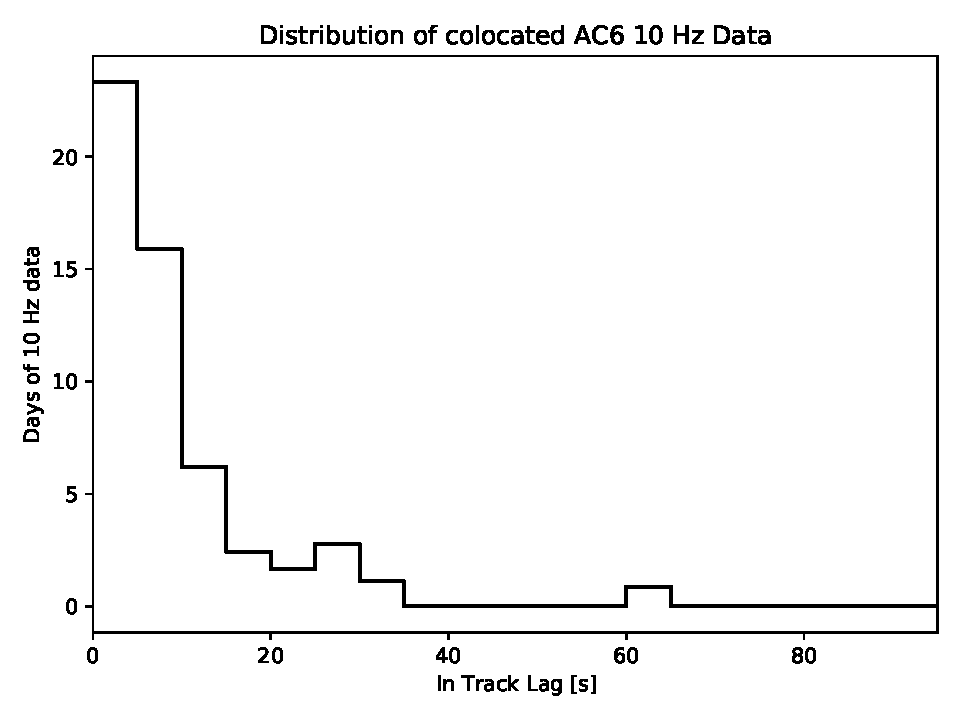
\includegraphics[width=\textwidth]{a_10hz_dist.pdf}
\caption{The distribution of colocated 10 Hz data as a function of in-track lag. Bins are 5 kilometers wide.}
\label{a_10Hz_dist}
\end{figure}

\section{Curtain Width Examples}
We defined the curtain width in the dos1 time series as the width at half of the curtain's topographic prominence. Topographic prominence for a time series is the height of a peak relative to the maximum of the two minimums on either side of the peak, located somewhere between the peak and any higher peak. Figure \ref{a_topographic_prominence} shows 5 examples of curtains observed by AC6A in red (for clarity the AC6B data is not shown), and the curtain width is shown by the horizontal black line.

\begin{figure}
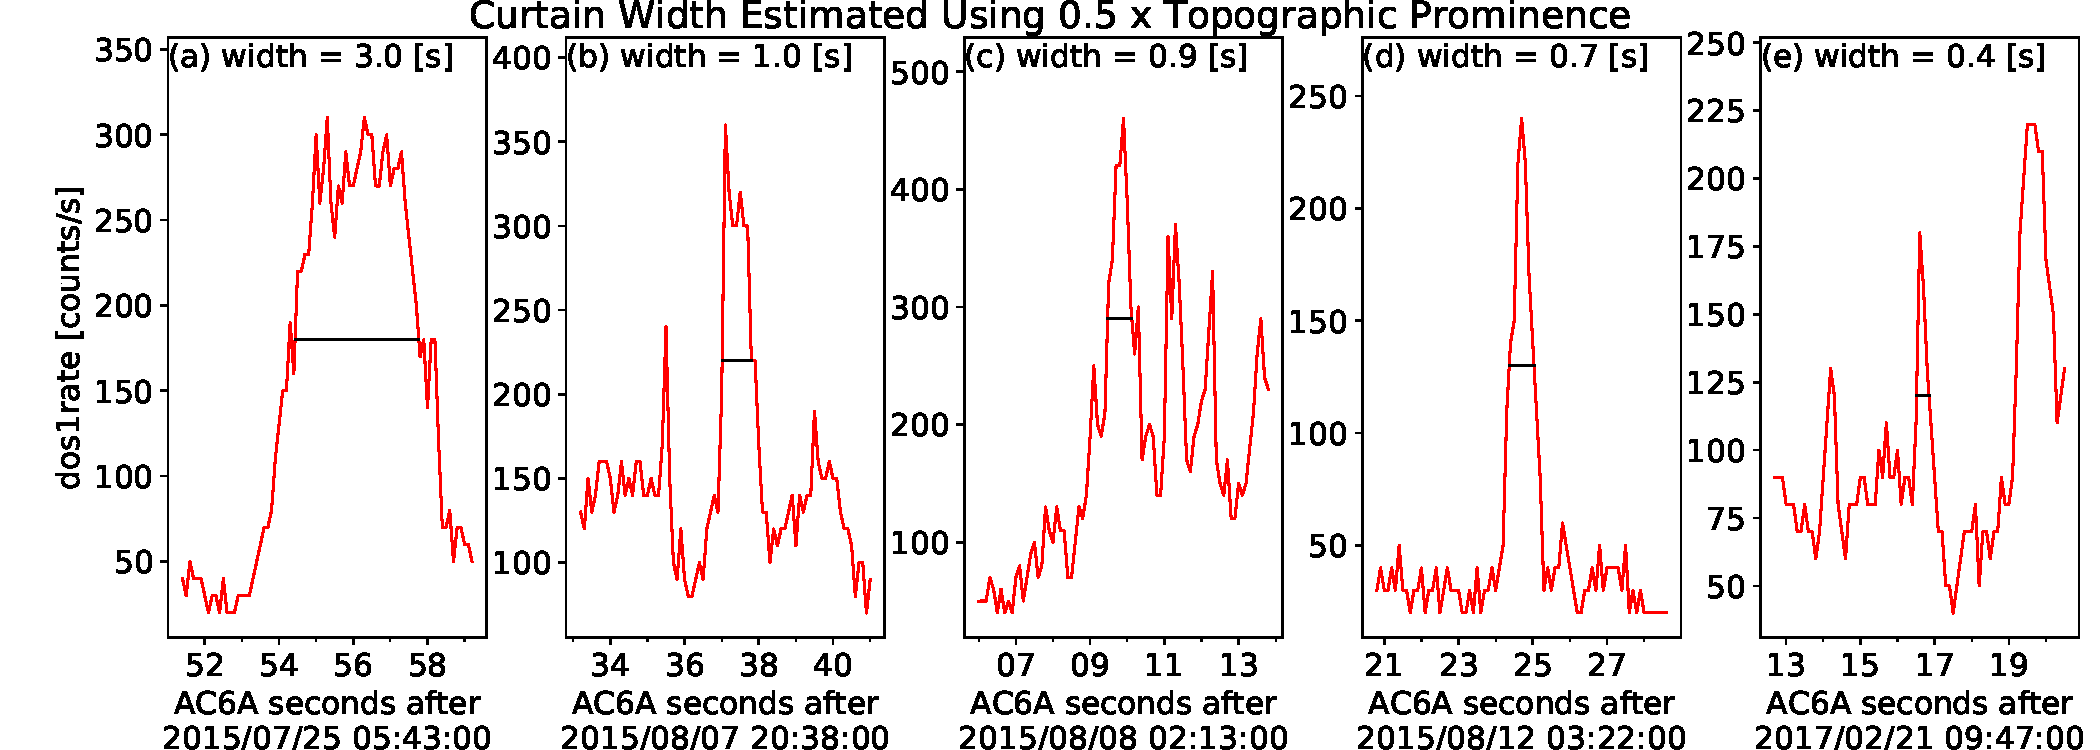
\includegraphics[width=\textwidth]{a_topographic_prominence.pdf}
\caption{Five examples of curtains observed by AC6A shown with the red curves and the curtain widths are shown with the horizontal black lines. The height of the horizontal black lines are at half of the curtain's topographic prominence.}
\label{a_topographic_prominence}
\end{figure}

\acknowledgments
This work was made possible with the help from the many engineers and scientists at The Aerospace Corporation who designed, built, and operated AC6. M. Shumko was supported by NASA Headquarters under the NASA Earth and Space Science Fellowship Program - Grant 80NSSC18K1204 and NASA Postdoctoral Program at the NASA's Goddard Space Flight Center, administered by Universities Space Research Association under contract with NASA. D.L. Turner is thankful for support from the Van Allen Probes mission and a NASA grant (Prime award number: 80NSSC19K0280). The work at The Aerospace Corporation was supported in part by RBSP-ECT funding provided by JHU/APL contract 967399 under NASA's Prime contract NAS501072. The AC6 data is available at http://rbspgway.jhuapl.edu/ac6 and the IRBEM-Lib version used for this analysis can be downloaded from https://sourceforge.net/p/irbem/code/616/tree/.

\bibliography{/home/mike/Dropbox/0_firebird_research/A_presentations/refs}
%\bibliography{"refs"}

\end{document}